\subsection{프로그래밍}

컴퓨터 프로그램이란 컴퓨터가 특정 작업을 수행하도록 지시하기 위한 명령어의 집합이다. 많은 개인들이 다양한 종류의 문제를 해결하기 위해 프로그램을 작성하기 때문에, 고급 컴퓨터 언어들은 아주 다양한 기능들을 가지고 있다. 어떤 공학자들은 특정 작업을 수행하기 위해서 컴퓨터 언어가 가지고 있는 모든 기능을 섭렵하여야 하지만, 대부분의 사람들은 공학적 응용 위주의 수치계산을 수행할 수 있을 정도면 충분하다.

\begin{itemize}
\item 단순한 정보의 표현[상수, 변수, 형식 선언(type declarations)]
\item 효과적인 정보의 표현[데이터 구조, 배열(array), 기록(record)]
\item 수학적 공식[지정(assignment), 우선순위 규칙(priority rule), 기본적 함수(intrinsic function)]
\item 입력/출력
\item 논리적 표현[순차적 진행(sequence), 선택 및 조건분기(selection), 반복(repetition)]
\item 모듈프로그래밍(module programming)[함수(function), 서브루틴(subroutine)]
\end{itemize}

\subsubsection{구조화된 프로그램(structured program)}
구조적 프로그래밍의 주요 아이디어는 어떤 수치알고리즘도 순차적 진행(sequence), 선택(selection), 반복(repetition)이라는 3개의 기본적 제어구조(control structure)로 이루어질 수 있다.

구조적 프로그래밍 혹은 프로그래밍에 있어 순서도(flowchart)는 알고리즘 논리의 이해를 돕지만, 본 강의에서는 다루지 않는다.

\subsubsection{논리적 표현}

\begin{itemize}
\item \textbf{순차적 진행(sequence)} 순차적 구조(sequence structure)는 한번에 하나의 명령을 수행함. 코딩에 있어 위에서 아래구문으로 수행됨
\item \textbf{선택(selection)} 순차적 구조의 프로그램의 흐름을 논리적 결정(logical condition)으로 분리하거나 분기시킴. (IF/IF-ELSE/CASE등)
\item \textbf{반복(repetition)} 명령을 반복적으로 수행하는 수단. 흔히 루프(loop)라고 불리는 구문은 decision loop이 일반적이고 반복 구문에서 조건에 의해 반복문을 빠져나가는 위치가 어디에 있는지에 따라 pretset loop, posttest loop으로 불리운다. 그러나 MATLAB은 while 구문으로 decision loop을 제어하며 그 확장성이 많이 좋은편은 아니다. 주로 횟수제어(for-loop)방식을 사용한다.
\end{itemize}

\subsection{모듈프로그래밍}

컴퓨터 프로그램은 각각 독립적을 개발되고 검증될 수 있는 여러개의 작은 부프로그램(subprogram)과 모듈(module)로 나눌 수 있다. MATLAB에서는 함수(function)이 그역할을 하며, 여러개의 입력변수에서 여러개의 출력변수를 내보내는등 독립적인 역할을 한다.
모듈프로그래밍은 여러가지 장점을 가지고 있다. 크기가 작고, 스스로 필요한 도구들을 갖춘 구성단위들을 이용하면 그 밑에 깔려있는 논리를 고안해내고, 개발자와 사용자 모두가 이를 쉽게 이해하게 된다. 각각의 모듈이 독립적이면서도 완벽하게 작동하기 때문에 프로그램의 개발 작업도 매우 쉽게 진전될 수 있다.

\subsection{라이브러리 \& 툴박스(Toolbox)}
본 강의에서 쓰일 MATLAB은 쉬운 대화식으로 프로그래밍되고, 행렬연산, 기호연산, 수치적 함수등을 포함하여 공학자들에게 매우 필요한 구조적인 프로그램이다. 그리고 수치해석이나 새로운 공학적 이슈들이 툴박스(Toolbox)의 형태로 배포된다.




%\begin{figure}[!hbpt]
%\centering
%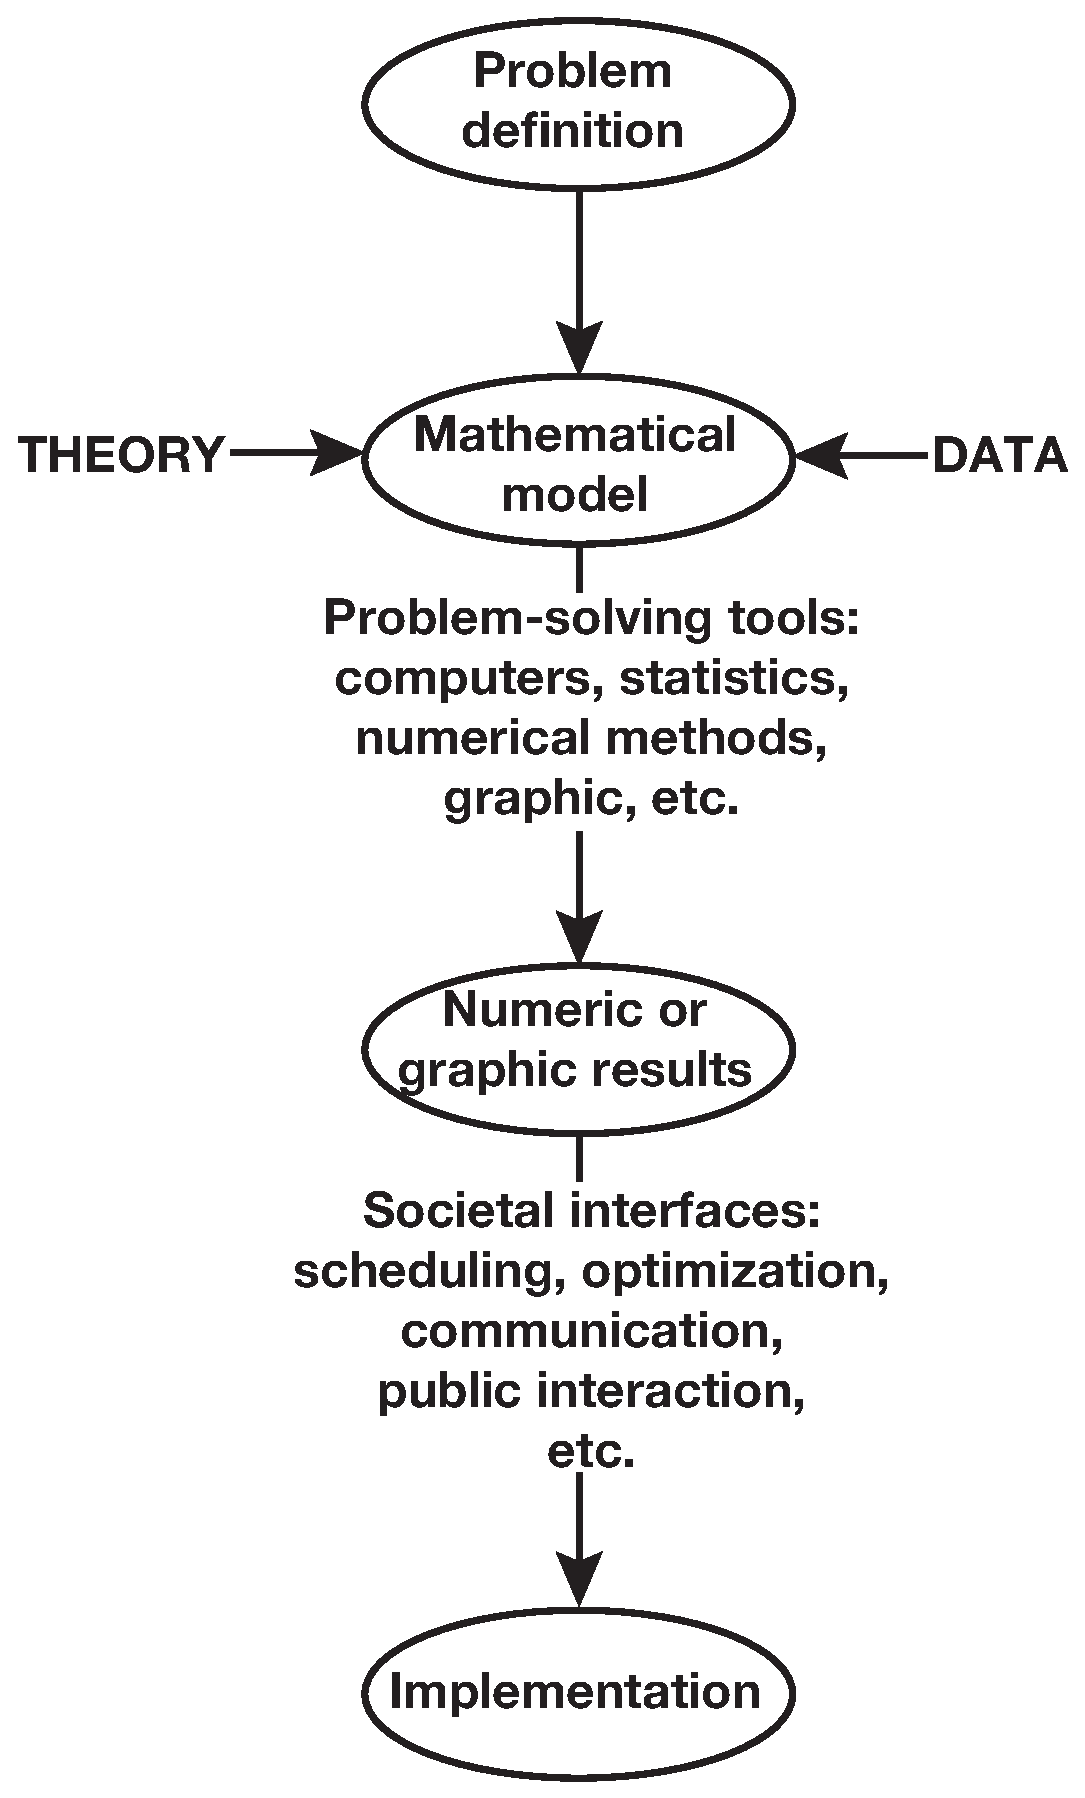
\includegraphics[keepaspectratio=true,width=0.5\linewidth]{figs/1-1.eps}
%\caption{공학적 문제의 해법과정}
%\label{fig:1-1}
%\end{figure}
%
%\clearpage
%\subsection{단순화된 수학적 모델}
%
%\begin{itemize}
%\item \textbf{수학적 모델(mathematical model)} 물리적 시스템이나 과정의 이해에 필수적으로 요구되는 특징을 수학적으로 표현한 함수의 관계식
%\begin{equation}
%종속변수=f\left(독립변수들, 매개변수들, 강제함수들\right)
%\label{eq:1-1}
%\end{equation}
%\item \textbf{종속변수(dependent variables)} 시스템의 거동이사 상태를 기술하는 특성량
%\item \textbf{독립변수(independent variables)} 시스템의 거동을 결정하는데 사용되는 시간과 공간과 같은 차원
%\item \textbf{매개변수(parameters)} 시스템의 성질이나 구성
%\item \textbf{강제함수(forcing functions)} 시스템에 작용되는 외부의 영향
%\end{itemize}
%식(\ref{eq:1-1})의 수학적 표현은, 단순한 대수적 관계식으로부터 매우 복잡한 연립미분방정식에 이르기까지 매우 다양한 적용범위를 가진다. 예를 들어, Newton은 그의 경험에 근거하여, 물체가 가지는 운동량의 시간에 따른 변화는 이에 작용되는 외력의 합과 같다는 제2 운동법칙을 공식화하였다.
%
%\begin{equation}
%F=ma
%\end{equation}
%여기서 $F$는 물체에 주어진 유효힘($N$ 또는 $kg\cdot m/s^2$)이며, $m$은 물체의 질량($kg$)이며 $a$는 가속도($m/s^2$)이다.
%특정한 물체에 $F$의 힘을 가했을 경우 물체의 가속도 $a$는
%\begin{equation}
%a=\frac{F}{m}
%\label{eq:1-3}
%\end{equation}
%\begin{itemize}
%\item $a$ : 시스템의 거동을 기술하는 종속변수(dependent variable)
%\item $F$ : 시스템에 작용되는 외력을 나타내는 강제함수(forcing function)
%\item $m$ : 시스템의 특성을 나타내는 매개변수(parameter)
%\end{itemize}
%\textbf{$a$는 시간에따라 공간상에서 어떻게 변화할 것인가?}\\
%식(\ref{eq:1-3})은 물리적 시스템을 기술하는 전형적인 수학적 모델이다.
%\clearpage
%\subsubsection{해석해(analytic solution) 예제}
%\paragraph{낙하산병 문제로 정확해(exact solution) 구하기}
%
%\begin{figure}[!hbpt]
%\centering
%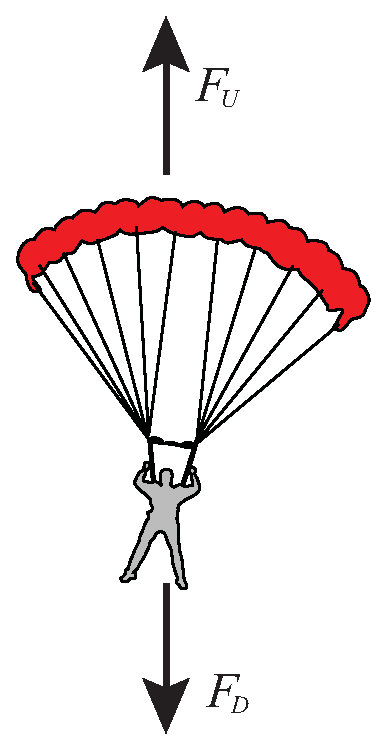
\includegraphics[keepaspectratio=true,width=0.2\linewidth]{figs/parachute.eps}
%\caption{낙하산병에 작용하는 힘에 대한 개략도. $F_D$는 중력에 의해 아래로 작용하는 힘이고, $F_U$는 공기의 저항에 의하여 위로 작용하는 힘이다.}
%\label{fig:1-2}
%\end{figure}
%
%\begin{equation}
%\frac{dv}{dt}=\frac{F}{m}
%\end{equation}
%
%\begin{equation}
%F=F_{D}+F_{U}
%\end{equation}
%
%\begin{equation}
%F_{U}=-cv
%\label{eq:1-7}
%\end{equation}
%
%\begin{equation}
%\frac{dv}{dt}=\frac{mg-cv}{m}
%\label{eq:1-6}
%\end{equation}
%
%\begin{equation}
%\frac{dv}{dt}=g-\frac{c}{m}v
%\label{eq:1-7}
%\end{equation}
%
%식~\ref{eq:1-6} 혹은 식~\ref{eq:1-7}의 엄밀해(exact solution)을 구하기 위해서는 미분방정식의 \textbf{변수분리(separation of variables)}\footnote{종속변수에 관련된 항과 독립변수에 관련된 항을 분리시킬 수 있을 때, 그 각각의 변수에 관해 적분하여 해를 구하는 미분방정식 풀이법의 일종} 방법등이 사용되어야 한다.
%
%\begin{equation}
%\frac{m}{mg-cv}dv=1\cdot dt
%\label{eq:1-8}
%\end{equation}
%
%양변을 적분하면 식(\ref{eq:1-8})은 시각 $T$에서 다음과 같이 변형할 수 있다.
%
%\begin{equation}
%\int_{v(0)}^{v(T)}\frac{m}{mg-cv}dv=\int_{0}^{T}1\cdot dt
%\label{eq:1-9}
%\end{equation}
%
%초기속도가 $0$ 즉, $t=0$일때, $v(0)=0$로 가정하고, $mg-cv$를 시간의 종속변수$X$로 치환하면,
%\begin{eqnarray}
%mg-cv=X\\
%\frac{dX}{dv}=-c\\
%dv=-\frac{1}{c}dx
%\end{eqnarray}
%
%치환변수 $X$의 초기값과 $T$에서의 값은 각각, $X(0)=mg$ 그리고 $X(T)=mg-cv(T)$가 된다. 다시 식(\ref{eq:1-9})에 대입하면,
%
%\begin{equation}
%-\frac{m}{c}\int_{X(0)}^{X(T)}\frac{1}{X}dv=\int_{0}^{T}1\cdot dt
%\label{eq:1-10}
%\end{equation}
%
%식(\ref{eq:1-10})을 계산하면,
%
%\begin{equation}
%-\frac{m}{c}\ln X\arrowvert_{X(0)}^{X(T)}=T
%\end{equation}
%
%치환된 변수를 환원하면서 전개하면,
%
%\begin{equation}
%-\frac{m}{c}\left[\ln\left\{mg-cv(T)\right\}-\ln(mg)\right] = T
%\end{equation}
%
%정리하면
%
%\begin{equation}
%\ln\left(1-\frac{c}{mg}v(T)\right) = -\frac{c}{m}T\\
%\end{equation}
%
%양변에 $\ln$을 취하면,
%
%\begin{equation}
%e^{-(c/m)T}=1-\frac{c}{mg}v(T)
%\end{equation}
%
%결국 시각 $T$에서 엄밀해는 식(\ref{eq:1-11})과 같이 계산된다.
%
%\begin{equation}
%v(T)=\frac{mg}{c}\left(1-e^{-(c/m)T}\right)
%\label{eq:1-11}
%\end{equation}
%
%\begin{figure}[!hbpt]
%\centering
%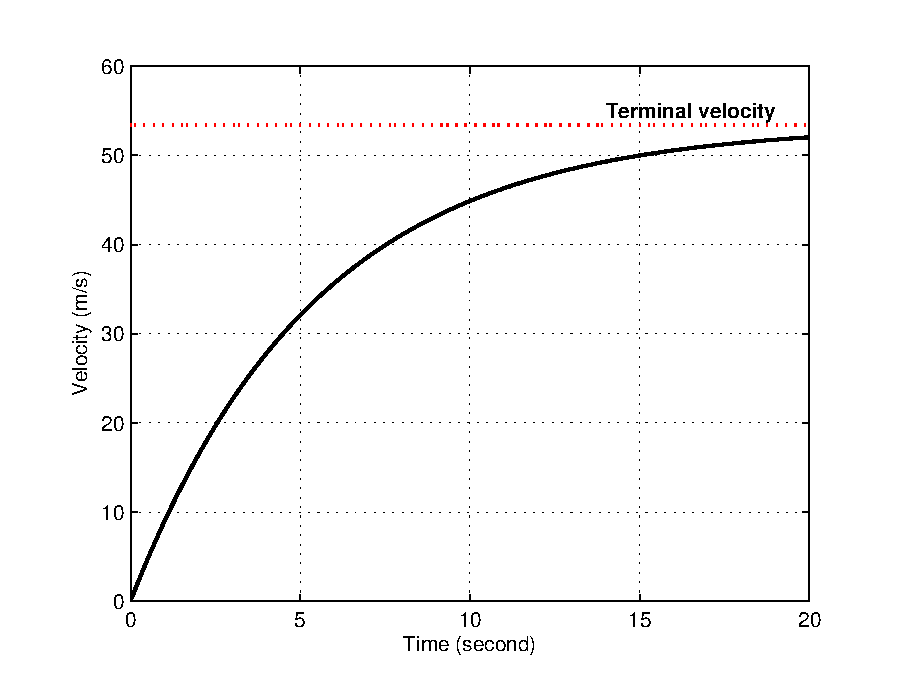
\includegraphics[keepaspectratio=true,width=0.4\linewidth]{figs/1-3.eps}
%\caption{낙하산병 문제의 해석해, 시간에 따라 속도가 증가하여 종단속도로 접근}
%\label{fig:1-3}
%\end{figure}
%
%\clearpage
%\subsubsection{수치해법(numerical method) 예제)}
%
%수치해법은 단순히 산술연산을 이용하여 해를 얻을 수 있도록 수학적 문제를 재공식화 하는 것이다. 근사화 문제를 생각하면 시간의 증분 즉, $\Delta$가 유한하기 때문에 $dv/dt \cong \Delta v/ \Delta t$는 근사식이 된다. 미적분학에서는
%
%\begin{equation}
%\frac{dv}{dt}=\lim_{\Delta t \rightarrow 0} \frac{\Delta v}{\Delta t}
%\end{equation}
%
%앞서 세운 수학적 모델 식(\ref{eq:1-7})를 생각해보면 다음과 같이 근사화 될 수 있다.
%\begin{equation}
%\frac{dv}{dt} \cong \frac{\Delta v}{\Delta t} = \frac{v\left(t_{i+1}\right)-v\left(t_{i}\right)}{t_{i+1}-t_{i}} = g-\frac{c}{m}v\left(t_{i}\right)
%\label{eq:1-11}
%\end{equation}
%위의 식(\ref{eq:1-11})을 다시 정리하면
%\begin{equation}
%v\left(t_{i+1}\right)=v\left(t_{i}\right)+\left[g-\frac{c}{m}v\left(t_{i}\right)\right]\left(t_{i+1}-t_{i}\right)
%\end{equation}
%
%\begin{figure}[!hbpt]
%\centering
%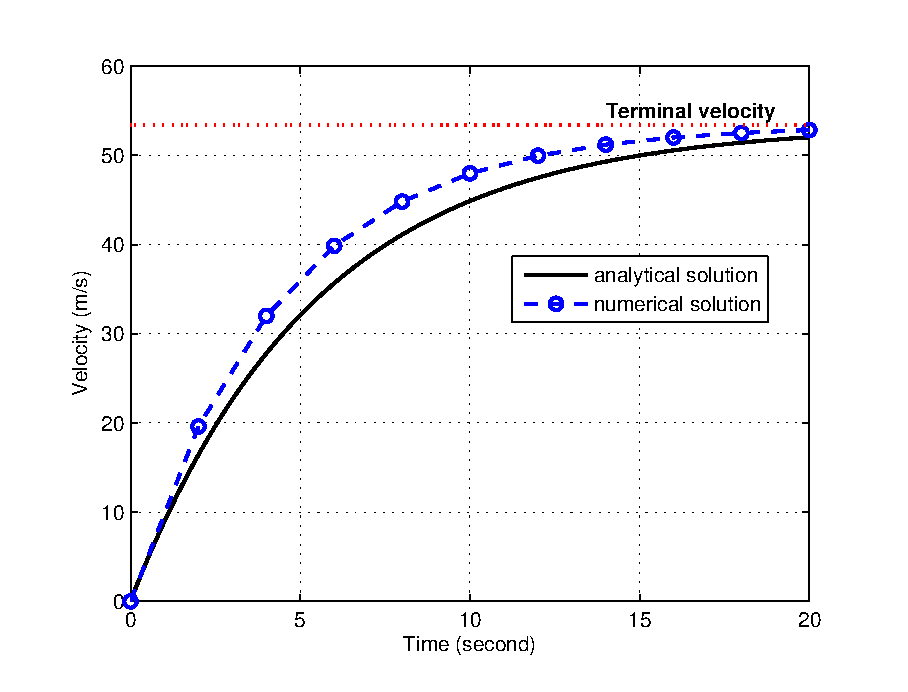
\includegraphics[keepaspectratio=true,width=0.6\linewidth]{figs/1-5.eps}
%\caption{낙하산병 문제에서의 수치해와 해석해의 비교}
%\label{fig:1-5}
%\end{figure}
%
%\paragraph{$\bigstar$테일러 급수(Taylor Series)}
%테일러 급수(Taylor Series)는 수치해석에서 매우 중요한 역할을 한다.(4장에서 학습)
%
%\begin{tabular}[c]{|p{4.7cm}|}
%\hline
%\textbf{Leonhard Euler 1707-1783}
%\begin{displaymath}
%e^{\pi i} +1=0
%\end{displaymath}
%\\\hline
%\end{tabular}
%
%\begin{tabular}[c]{|p{4.7cm}|}
%\hline
%\textbf{Isaac Newton 1642-1727}
%\begin{eqnarray*}
%e&=&1+\frac{1}{1!}+\frac{1}{2!}+\frac{1}{3!}+\cdots \\
%&\cong& 2.718281828459046 \cdots
%\end{eqnarray*}
%\\\hline
%\end{tabular}
%
%\begin{law}
%$n\geq0$인 정수 $n$에 대하여, 폐구간$[a,x]$에서 $n$번 미분가능하고 개구간$(a,x)$에서 $(n+1)$번 미분가능한 함수$f$는
%\begin{displaymath}
%f(x)=\sum_{n=0}^{\infty}\frac{f^{(n)}(a)}{n!}(x-a)^{n}
%\end{displaymath} 
%로 나타내어질 수 있다. 처음 몇 항까지를 선택함으로써 $x=a$주변에서의 $f(x)$의 근사식으로 사용할 수 있는데, 이를 \textbf{테일러 다항식(Taylor polynomial)}이라고 한다. 특히 \textbf{선형근사}는 $n=1$인 테일러 급수로 볼 수 있다. $a=0$인 경우를 특별히 \textbf{맥로린 급수(Maclaurin series)}라고 부른다.
%\end{law}
%
%\framebox[1.1\width]{과제1 (제출기한 9월18일)}
%
%\begin{itemize}
%\item[1] 초기속도 $v(0)$가 $0$이 아닌 경우, $v(0)$ 상수를 도입하여 정밀해를 구하라
%\item[2] 낙하하는 낙하산병에게 작용하는 힘을 계산하는 과정에서, 식(\ref{eq:1-7})로 주어진 선형관계식 대신, 다음과 같은 2차식을 사용하여 정밀해 혹은 수치해를 구하여라
%\begin{displaymath}
%F_{U}=-c'v^2
%\end{displaymath}
%단, $c'$은 2차항력계수($kg/m$)이며, 수치해를 구할땐, 10초후의 낙하산병의 속도를 구하라. 여기서, 낙하산병의 질량은 68.1kg이고 2차항력계수는 $0.232kg/m$이다.
%\item[3] 테일러급수(Taylor series)를 증명하라.
%%\item[4] 정확도(accuracy)와 정밀도(precision)에 대하여 조사하라\footnote{\url{http://en.wikipedia.org/wiki/Accuracy_and_precision}} 그리고 각 전공영역에 맞추어  특정한 공학적 이슈를 예를들어 불확실성(uncertainty)에 대하여 자신의 생각을 쓰시오.
%\end{itemize}